\section{Resultados}
\label{sec:resultados}

Apresentam-se a caracterização dos sensores, a avaliação nas capturas
integradas e a validação com motor ativo. A feira de ciências é relatada
separadamente, sem resultados quantitativos. O desfecho principal é detectar
postura prejudicial por alerta ativo ou inativo; identificar a classe de
postura é uma informação complementar.

\subsection{Caracterização dos sensores em bancada}
\label{sec:res-bancada}

\subsubsection{Orientação do tronco e referência individual}

Na bancada do IMU, com um participante e sem o suporte final do colar, a
principal sobreposição ocorreu entre curvar o tronco e abaixar a cabeça:
distância entre centroides de aproximadamente $6{,}9\degree{}$, contra pelo
menos $21{,}7\degree{}$ nos demais pares. A
Figura~\ref{fig:res-imu-bancada} retoma a variação da referência entre
montagens. A sobreposição limita a classificação dessas duas
posturas prejudiciais, mas não impede, por si só, sua detecção binária.

\begin{figure}[H]
  \centering
  \caption{Mudança da referência de ereto entre remontagens do IMU na
  campanha de bancada.}
  \label{fig:res-imu-bancada}
  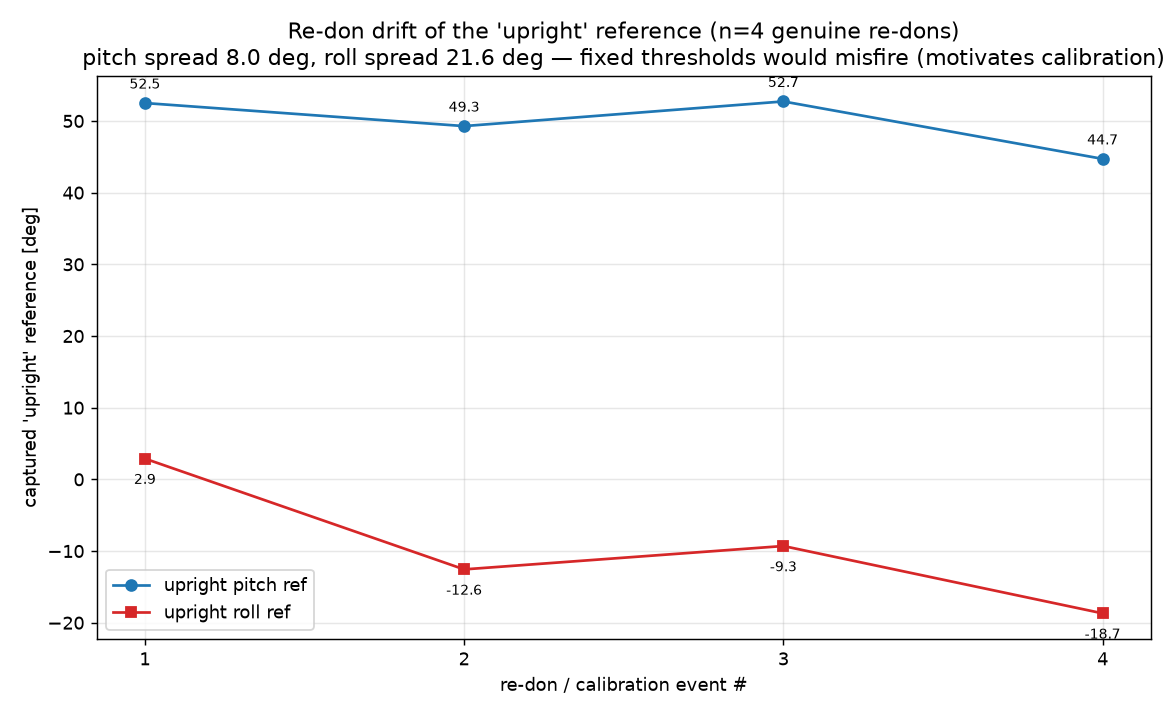
\includegraphics[width=0.80\linewidth]{04_redon_drift.png}
  \fonte{Elaborado pelo autor (2026)}
\end{figure}

Nas quatro épocas genuínas de retirada e recolocação, a referência de ereto
variou aproximadamente $8{,}0\degree{}$ em \textit{pitch} e $21{,}6\degree{}$
em \textit{roll}, valores comparáveis ou superiores ao desvio a detectar.
Isso sustenta a calibração individual em ereto. Trata-se de mudança da
montagem e da referência, não de deriva por integração do giroscópio: os
ângulos são estimados pelo acelerômetro.

O percentil 95 do módulo do desvio em ereto foi $6{,}4\degree{}$; o
percentil 5 agregado das posturas inadequadas foi $18{,}6\degree{}$.
O limiar inicial de $10\degree{}$ separou esses regimes, sem falso alarme e
com detecção de todas as posturas inadequadas nessa base. O resultado é
restrito a um participante e a movimentos pronunciados. As capturas
integradas mostram margens menores e falhas ausentes na bancada; a
orientação dos eixos na montagem final é indicada na
Seção~\ref{sec:res-capturas}.

\subsubsection{Resposta dos FSR402 e uso como pressão relativa}

A resistência do FSR1 caiu de aproximadamente 4134\,\ohm{} em
50\,g para 180\,\ohm{} no limite de aproximadamente 2\,kg da
balança. A maior redução ocorreu abaixo de 1{,}2\,kg. A curva se achatou,
mas continuou decrescendo: os valores de $160$--180\,\ohm{} nessa faixa
não representam um piso calibrado.

O ajuste por lei de potência apresentou $R^2$ de aproximadamente
$0{,}95$--$0{,}97$. A condutância, $G=1/R$, foi aproximadamente linear em
relação à carga, com $R^2$ próximo de $0{,}95$, superior ao ajuste linear da
própria resistência, próximo de $0{,}43$. A Figura~\ref{fig:res-fsr-modelo}
reproduz a comparação dos modelos e a estimativa de resolução da bancada.
A estimativa de cerca de 3\,\ohm{} por contagem em baixa resistência
corresponde ao ADC de 10 bits utilizado naquela etapa; não é a resolução do
circuito final, que lê contagens de 12 bits no XIAO.

\begin{figure}[H]
  \centering
  \caption{Modelos da resposta do FSR402 e resolução estimada na montagem de
  bancada da entrega parcial.}
  \label{fig:res-fsr-modelo}
  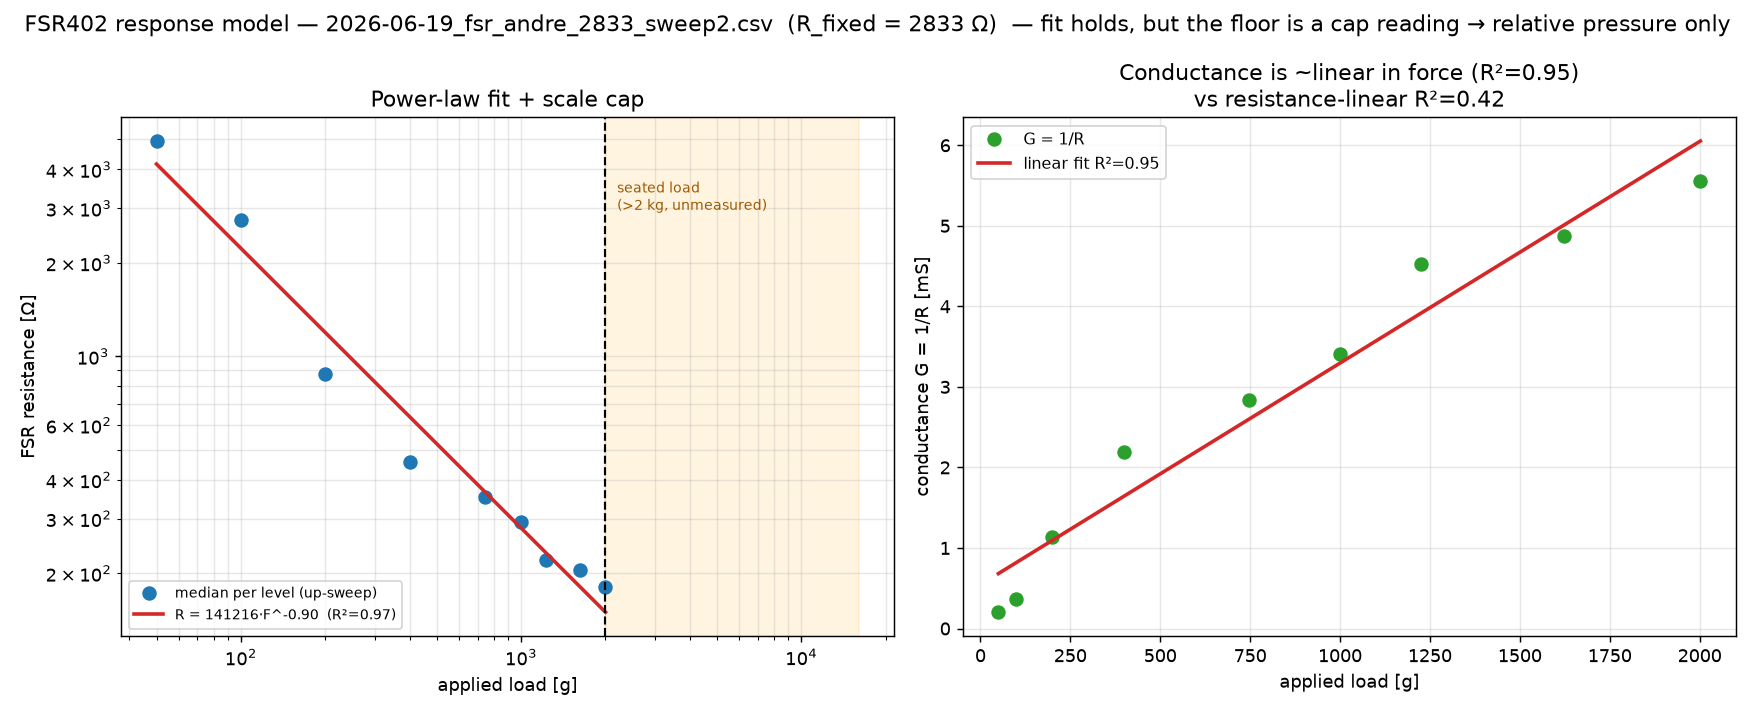
\includegraphics[width=0.96\linewidth]{fsr_model.png}
  \fonte{Elaborado pelo autor (2026)}
\end{figure}

A dependência do histórico de carga foi mais acentuada no regime leve. No
FSR2, a diferença entre descarga e carga passou de aproximadamente
$-76\,\%$ em 50\,g para $-6\,\%$ em 1\,kg. A histerese média
absoluta foi próxima de $52\,\%$ até 400\,g e de $6\,\%$ a partir de
1\,kg. Sob carga constante de 1\,kg, a resistência variou
$-7{,}4\,\%$ no FSR1 em cerca de 11 minutos e $-11{,}5\,\%$ no FSR2 em
cerca de 12 minutos. O \textit{creep} e a histerese impedem tratar cada
leitura como uma medida estável de força absoluta, mesmo que a direção da
resposta seja consistente.

A comparação entre três sensores, na Figura~\ref{fig:res-fsr-pecas}, mostrou
variações entre peças de aproximadamente $10$--$46\,\%$, conforme a carga.
Por exemplo, as medianas em 400\,g foram $453$, $514$ e 502\,\ohm{};
em 1\,kg, foram $290$, $267$ e 391\,\ohm{}. Variações maiores,
de três a onze vezes, apareceram em um transiente de acomodação do aplicador
rígido sobre um sensor. Esse transiente foi identificado como efeito da
montagem e excluído da comparação entre peças. Ele evidencia sensibilidade
à forma de aplicação da carga, mas não quantifica a variação de um FSR
instalado na espuma de uma cadeira sob um usuário.

\begin{figure}[H]
  \centering
  \caption{Variação entre três FSR402 nas varreduras de carga; os pontos
  associados à acomodação inadequada não representam dispersão entre peças.}
  \label{fig:res-fsr-pecas}
  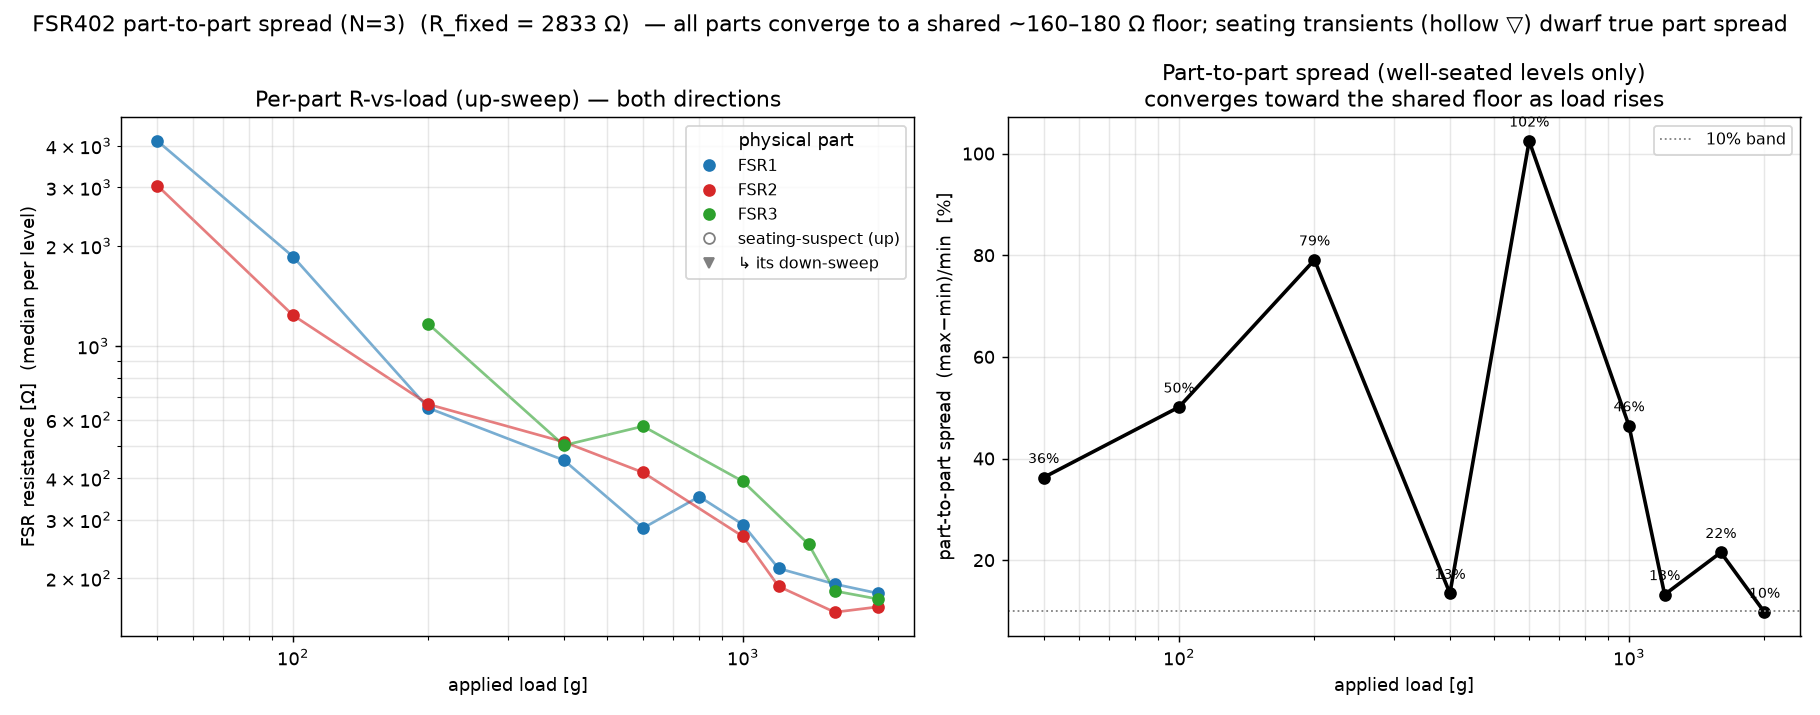
\includegraphics[width=0.94\linewidth]{fsr_parttopart.png}
  \fonte{Elaborado pelo autor (2026)}
\end{figure}

Esses resultados sustentam o uso dos FSRs como pressão relativa e contato.
A regra final utiliza somas de leituras cruas de grupos do assento e sua
relação com a linha de base individual, sem converter contagens em força.
A condutância auxilia a interpretação e a visualização; a decisão não exige
uma curva de força ajustada por sensor.

\subsection{Capturas do sistema completo em 21 de outubro de 2026}
\label{sec:res-capturas}

\subsubsection{Composição do conjunto de dados}

O conjunto integrado contém nove arquivos de oito participantes, com duas
sessões de André e uma de cada um dos demais participantes. Foram registradas
127773 amostras, em aproximadamente $106{,}5$ minutos de gravação. A
Tabela~\ref{tab:res-capturas} apresenta as durações por arquivo. O tempo com
presença estimada no assento foi de aproximadamente $103{,}5$ minutos;
transições, ajustes e intervalos sem etiqueta explicam por que esse tempo é
maior que o utilizado para pontuar as posturas.

\begin{table}[H]
  \centering
  \caption{Composição das nove capturas do sistema completo em 21/10/2026.}
  \label{tab:res-capturas}
  \begin{singlespace}
  \small
  \begin{tabularx}{\linewidth}{Xrrrr}
    \toprule
    Participante / sessão & Registro & Presença & Avaliado & Segmentos \\
                          & (min) & (min) & (min) & \\
    \midrule
    André / 1       & $5{,}62$  & $5{,}32$  & $2{,}71$  & 9 \\
    André / 2       & $23{,}87$ & $22{,}46$ & $10{,}92$ & 23 \\
    Felipe          & $8{,}36$  & $8{,}27$  & $3{,}35$  & 10 \\
    Gustavo         & $12{,}75$ & $12{,}63$ & $5{,}96$  & 16 \\
    Rafael          & $9{,}41$  & $9{,}12$  & $5{,}13$  & 11 \\
    Ryan            & $18{,}61$ & $18{,}40$ & $7{,}42$  & 18 \\
    Thiago Fita     & $13{,}07$ & $12{,}60$ & $7{,}68$  & 16 \\
    Thiago M.       & $7{,}25$  & $7{,}20$  & $3{,}87$  & 10 \\
    Vinicius        & $7{,}55$  & $7{,}53$  & $3{,}71$  & 10 \\
    \midrule
    Total           & $106{,}48$ & $103{,}54$ & $50{,}74$ & 123 \\
    \bottomrule
  \end{tabularx}
  \fonte{Elaborado pelo autor (2026)}
  \end{singlespace}
  \par\smallskip
  {\footnotesize Registro: diferença entre o último e o primeiro instante de
  cada arquivo. Presença: soma dos quatro FSRs do assento de pelo menos 2000
  contagens. Avaliado: amostras rotuladas, sob calibração válida, após excluir
  os primeiros 2\,s de cada segmento. Presença e tempo avaliado são estimados
  pelo número de amostras dividido por 20\,Hz; totais calculados antes do
  arredondamento.}
\end{table}

Foram aproveitados 123 segmentos, correspondentes a 3044{,}6\,s de
amostras estabilizadas. Desses segmentos, 62 representam posturas para as
quais se espera alerta, 39 representam ereto ou reclinado e 22 representam
pernas cruzadas, que não devem gerar alerta na versão avaliada. O número de
segmentos e o tempo por postura constam na Tabela~\ref{tab:res-posturas}.
Os códigos de postura desta campanha diferem dos utilizados na bancada de
junho; os números apresentados a seguir correspondem às etiquetas de outubro.

\begin{table}[H]
  \centering
  \caption{Distribuição dos segmentos e do tempo avaliado por postura.}
  \label{tab:res-posturas}
  \begin{singlespace}
  \begin{tabularx}{\linewidth}{cXrrc}
    \toprule
    Código & Postura & Segmentos & Tempo (s) & Alerta esperado \\
    \midrule
    1 & Ereto                 & 27 & $532{,}10$ & Não \\
    2 & Curvado à frente      & 13 & $301{,}80$ & Sim \\
    3 & Cabeça à frente       & 12 & $283{,}35$ & Sim \\
    4 & Escorregado           & 13 & $353{,}20$ & Sim \\
    5 & Inclinado à esquerda  & 12 & $326{,}95$ & Sim \\
    6 & Inclinado à direita   & 12 & $318{,}25$ & Sim \\
    7 & Reclinado             & 12 & $314{,}10$ & Não \\
    8 & Perna E sobre D       & 11 & $324{,}60$ & Não \\
    9 & Perna D sobre E       & 11 & $290{,}25$ & Não \\
    \midrule
      & Total                & 123 & $3044{,}60$ & \\
    \bottomrule
  \end{tabularx}
  \fonte{Elaborado pelo autor (2026)}
  \end{singlespace}
\end{table}

As sessões incluem ordens fixas, repetições, recalibrações e roteiros
abreviados ou embaralhados. Rafael não realizou as posturas 3 e 7.
As sessões de André foram mantidas juntas no LOSO. Os critérios estão na
Seção~\ref{sec:metodologia}. São dados exploratórios, sem estatística
inferencial nem ensaio de uso prolongado em trabalho de escritório.

\subsubsection{O que os canais inerciais distinguem}

No colar final, \texttt{dpitch} representa principalmente movimento lateral
(positivo à direita), e \texttt{droll}, sagital (positivo para trás).
A Figura~\ref{fig:res-imu-posturas} mostra as medianas por sujeito e postura,
reunindo as amostras estabilizadas das sessões de cada participante.

A curvatura pronunciada para frente produziu medianas de \texttt{droll}
entre aproximadamente $-19{,}4\degree{}$ e $-52{,}3\degree{}$, com
separação em relação ao ereto em todos os participantes. A postura de cabeça
à frente apresentou sinais menores e mais variáveis: em Gustavo, Thiago M.
e Vinicius, as medianas sagitais ficaram entre $-4{,}6\degree{}$ e
$-7{,}5\degree{}$. Esses valores explicam por que o bom resultado de bancada
não se transferiu integralmente para movimentos mais localizados no pescoço.

As inclinações laterais inverteram o sinal de \texttt{dpitch}, como esperado,
mas sua amplitude variou. Na inclinação à esquerda, Felipe apresentou mediana
de apenas $-6{,}2\degree{}$, enquanto Rafael chegou a $-27{,}1\degree{}$.
Na inclinação à direita de Vinicius, a mediana foi de aproximadamente
$10{,}5\degree{}$, próxima ao limiar. Já reclinar e escorregar para frente
produziram, em geral, desvios sagitais positivos. Esse sinal isolado não
informa se o quadril continua apoiado na parte traseira do assento, diferença
que passou a ser fornecida pelos FSRs.

\begin{figure}[H]
  \centering
  \caption{Medianas dos desvios do IMU por postura e participante nas capturas
  integradas; os valores numéricos preservam a leitura sem cores.}
  \label{fig:res-imu-posturas}
  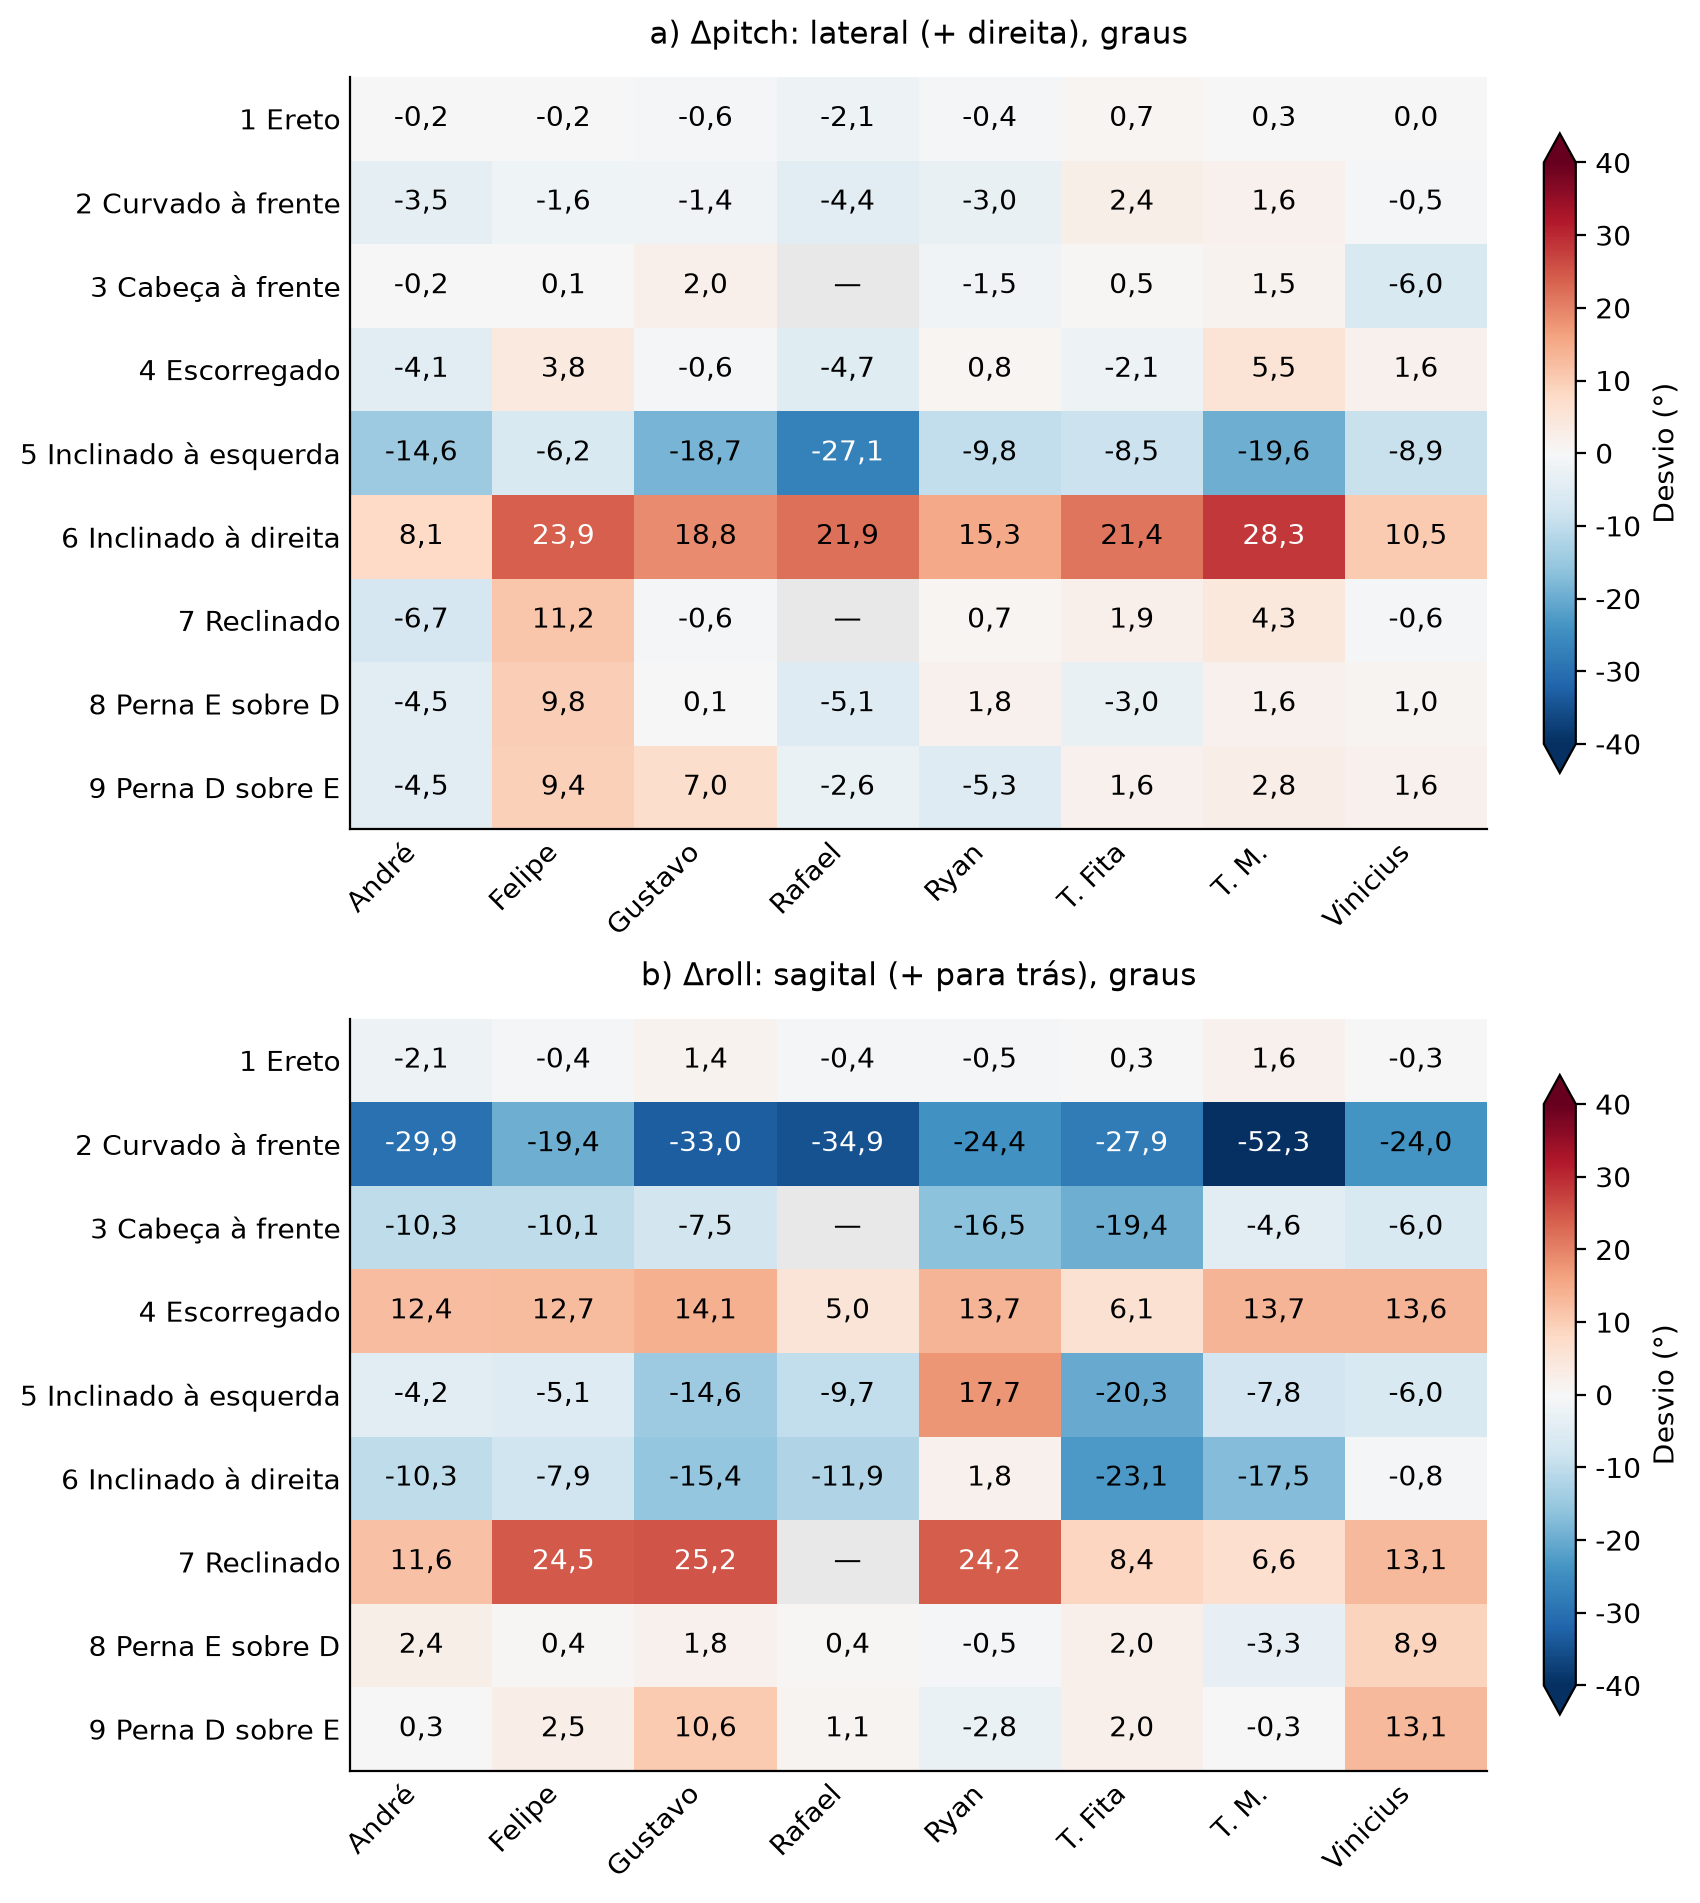
\includegraphics[width=\linewidth,height=0.76\textheight,keepaspectratio]{res_imu_posturas.png}
  \fonte{Elaborado pelo autor (2026)}
  \par\smallskip
  {\footnotesize E e D indicam esquerda e direita. T. Fita e T. M. são Thiago
  Fita e Thiago M. O traço indica postura não registrada, e não valor nulo.
  As escalas de cor são limitadas a $\pm40\degree{}$, mas as células mostram
  as medianas completas.}
\end{figure}

\subsubsection{Apoio traseiro e redistribuição lateral no assento}

A Figura~\ref{fig:res-assento-posturas} apresenta dois índices sem unidade:
a soma traseira dividida pela linha de base da calibração e a mudança do
índice esquerda/direita do assento em relação à mesma referência. A razão
traseira próxima de um indica apoio semelhante ao registrado em ereto; a
razão próxima de zero indica perda desse contato. No índice lateral, o sinal
positivo indica aumento relativo de leitura à esquerda. Essas grandezas
são razões de sinais elétricos, não frações calibradas do peso corporal.

Na postura escorregada, a mediana da razão traseira foi zero em 11 dos 13
segmentos. Os dois restantes apresentaram aproximadamente $0{,}23$ em uma
passagem de Thiago Fita e $0{,}49$ em Gustavo. Em contraste, no reclinado a
mediana agregada foi de aproximadamente $0{,}98$, com percentil 5 de
$0{,}65$. Portanto, os FSRs acrescentaram uma informação que o sentido da
inclinação do tronco não continha: a conservação ou perda de apoio do quadril.
No ereto, a razão traseira permaneceu entre $0{,}96$ e $1{,}09$ nos percentis
1 e 99 ao longo das sessões, cuja duração variou de cerca de 6 a 24 minutos.
Essa faixa ficou distante do limiar de escorregamento de $0{,}3$.

A redistribuição lateral foi menos uniforme que a perda de contato traseiro.
Em Felipe, a inclinação à esquerda combinou desvio inercial pequeno com
mediana de deslocamento lateral próxima de $+0{,}09$, suficiente para
confirmar a inclinação. Em Vinicius, a inclinação à direita produziu
aproximadamente $+0{,}04$, no sentido oposto ao esperado para essa postura,
impedindo a mesma confirmação. A mediana agregada também não descreve todas
as passagens: Ryan permaneceu escorregado durante uma inclinação à esquerda,
com perda de apoio traseiro, caracterizando uma postura mista.

Alguns canais inferiores do encosto permaneceram próximos de zero mesmo em
ereto, como em Rafael e Thiago M. Embora os oito FSRs sejam registrados,
a regra não utiliza razões individuais do encosto: seus índices decisivos
vêm dos grupos do assento. Não se demonstrou contribuição equivalente dos
oito pontos para o alerta.

\begin{figure}[H]
  \centering
  \caption{Medianas dos índices relativos do assento por postura e
  participante: apoio traseiro e deslocamento esquerda/direita.}
  \label{fig:res-assento-posturas}
  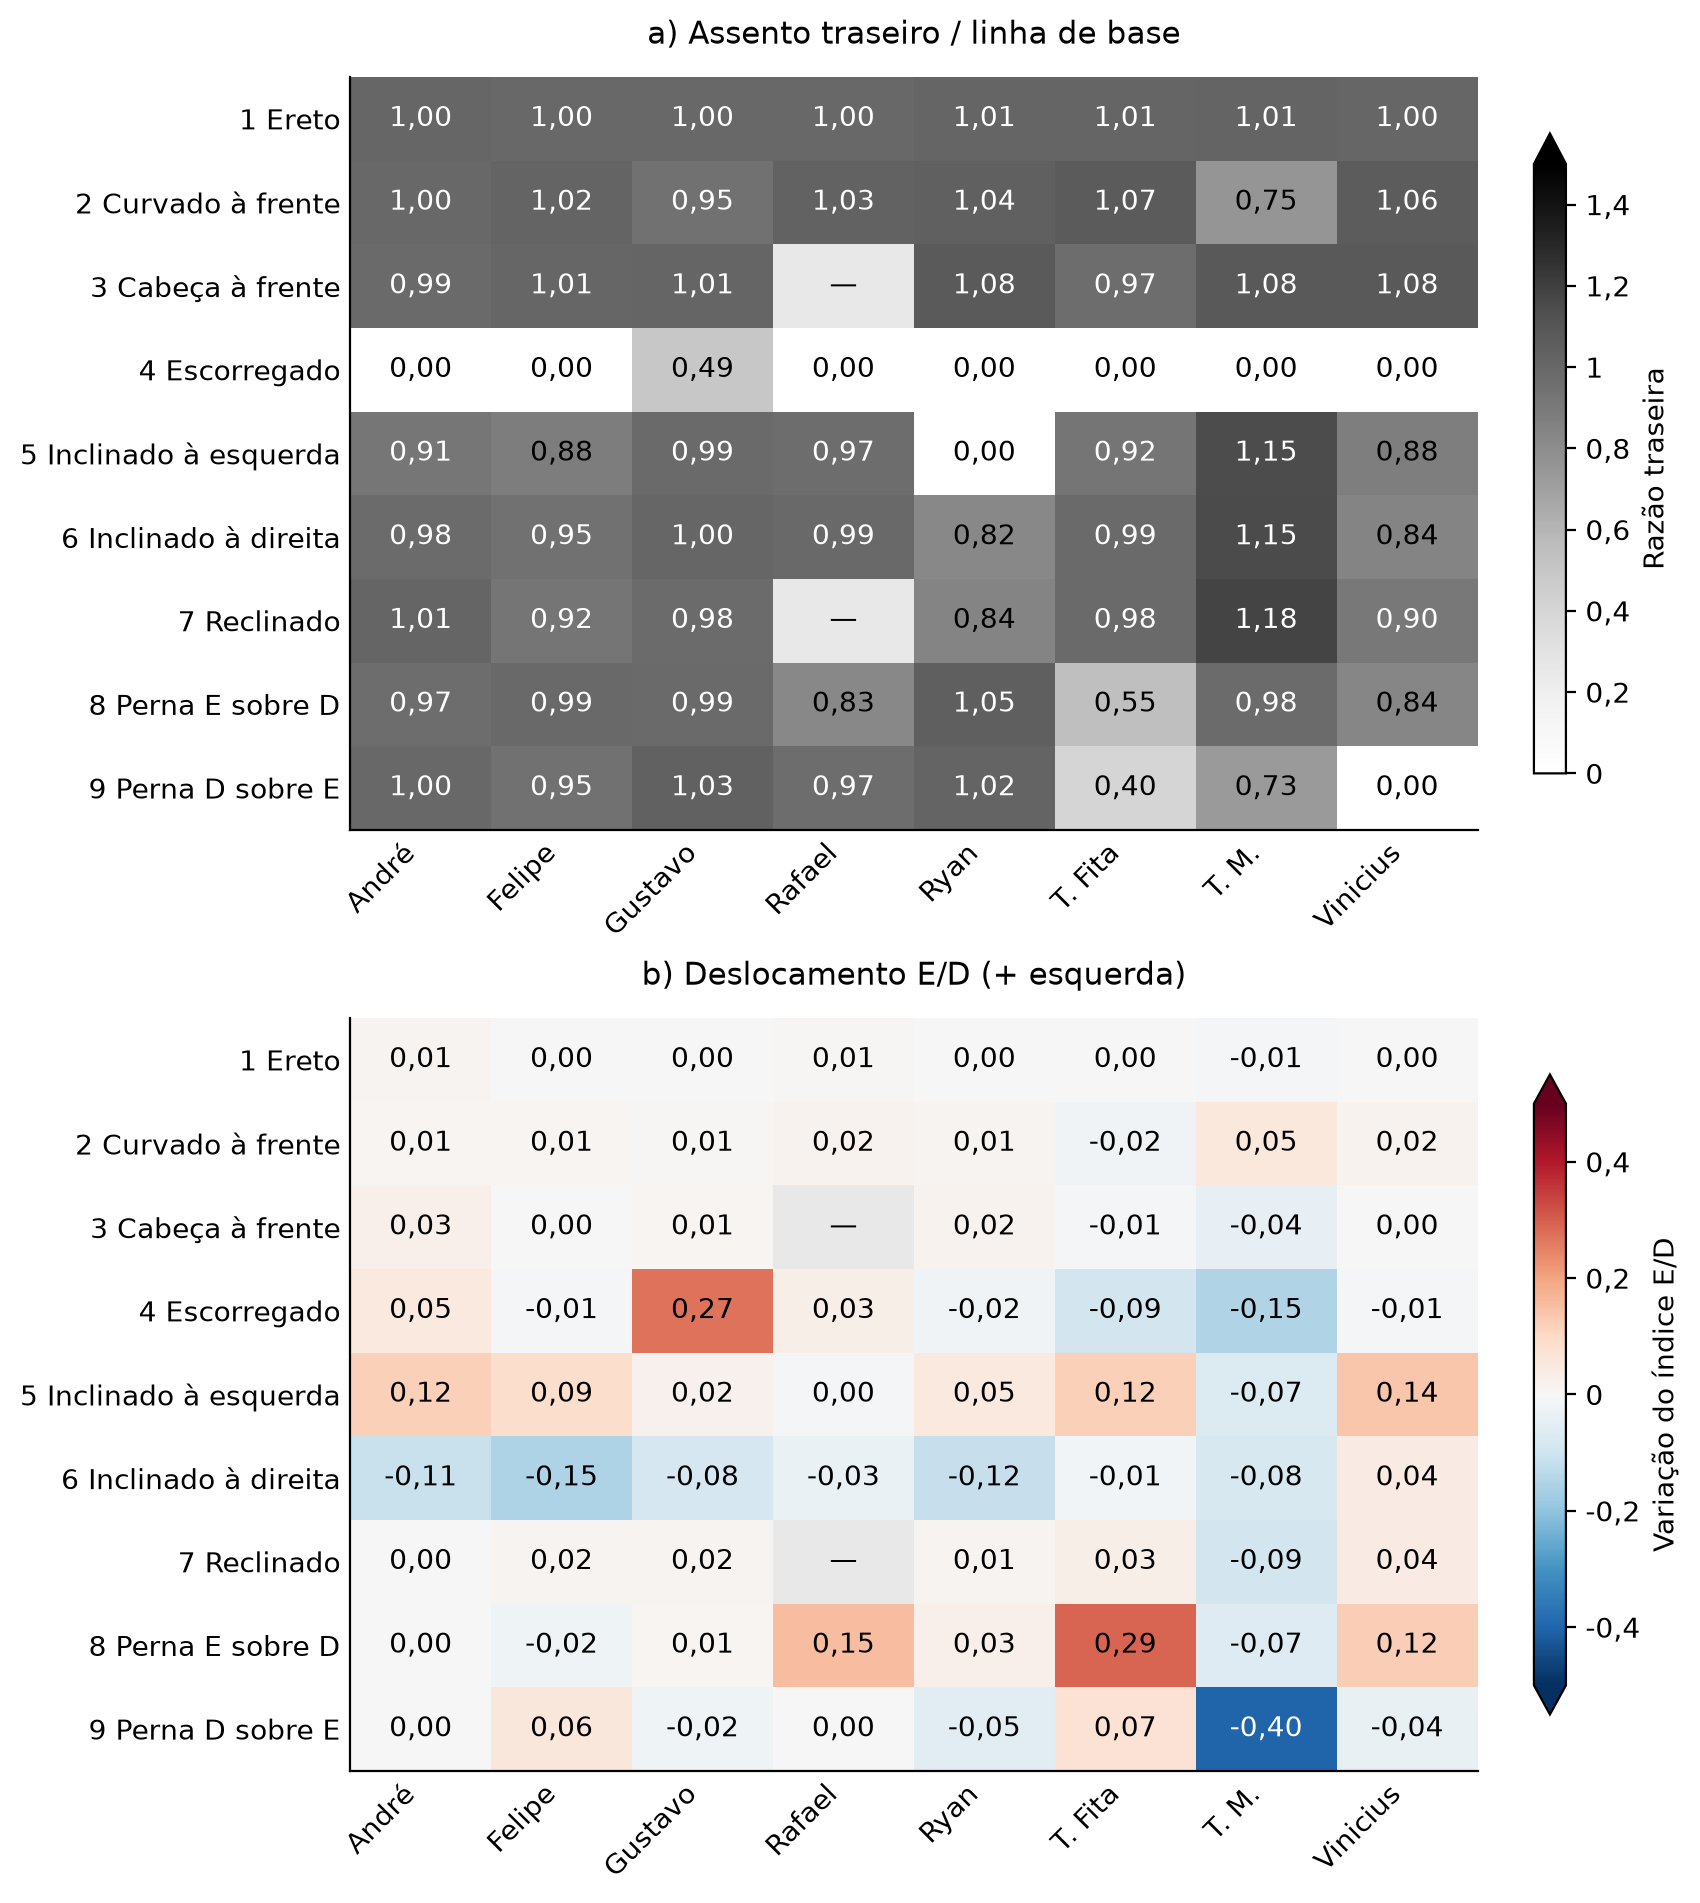
\includegraphics[width=\linewidth,height=0.76\textheight,keepaspectratio]{res_assento_posturas.png}
  \fonte{Elaborado pelo autor (2026)}
  \par\smallskip
  {\footnotesize Amostras estabilizadas sob calibração válida. O traço indica
  ausência de registro. Razão traseira igual a um e deslocamento lateral igual
  a zero correspondem à linha de base individual.}
\end{figure}

\subsection{Avaliação da regra de alerta}
\label{sec:res-alerta}

\subsubsection{Comparação global e avaliação LOSO}

A reprodução só-IMU concordou com o alerta original em
$99{,}74$--$100\,\%$ das amostras, conforme a sessão; diferenças pequenas
são compatíveis com ângulos arredondados próximos aos limiares.
Na Tabela~\ref{tab:res-comparacao}, a fusão final detectou 58/62 segmentos
prejudiciais, contra 55/62 da referência, elevando o tempo prejudicial
alertado de $84\,\%$ para $93\,\%$. O tempo ereto/reclinado alertado caiu de
$29\,\%$ para $2\,\%$. Percentuais de tempo ponderam as amostras;
a pontuação equilibra as frações por segmento conforme o protocolo.

\begin{table}[H]
  \centering
  \caption{Desempenho de detecção da referência só-IMU e da fusão nas capturas
  de 21/10/2026.}
  \label{tab:res-comparacao}
  \begin{singlespace}
  \small
  \begin{tabularx}{\linewidth}{Xccc}
    \toprule
    Indicador & Só-IMU & Fusão final & Fusão LOSO \\
    \midrule
    Segmentos prejudiciais com alerta & 55/62 & 58/62 & 58/62 \\
    Fração desses segmentos (\%) & 89 & 94 & 94 \\
    Tempo prejudicial com alerta (\%) & 84 & 93 & 92 \\
    Tempo ereto/reclinado com alerta (\%) & 29 & 2 & 3 \\
    Segmentos ereto/reclinado com alerta & 9/39 & 1/39 & 2/39 \\
    Tempo de pernas cruzadas com alerta (\%) & 10 & 11 & 28 \\
    Pontuação balanceada por segmento & $0{,}834$ & $0{,}935$ & $0{,}901$ \\
    \bottomrule
  \end{tabularx}
  \fonte{Elaborado pelo autor (2026)}
  \end{singlespace}
  \par\smallskip
  {\footnotesize Fusão final: parâmetros selecionados no conjunto completo.
  LOSO: resultado de cada sujeito com parâmetros selecionados sem seus dados.
  Segmento com alerta indica ao menos um alerta dentro do segmento, inclusive
  se iniciado antes da etiqueta. Percentuais arredondados ao inteiro.}
\end{table}

Em LOSO, a fusão conservou 58/62 segmentos detectados e $92\,\%$ do tempo
prejudicial alertado. O falso alarme foi de $3\,\%$ do tempo ereto/reclinado,
mas chegou a $28\,\%$ nas pernas cruzadas, avaliadas separadamente.
A pontuação caiu de $0{,}935$ para $0{,}901$, evidenciando a diferença entre
ajuste completo e transferência ao sujeito omitido. A referência só-IMU
não foi ajustada a essas capturas.

A execução de \texttt{analysis/fusion.py} reproduziu os totais da avaliação
documentada no repositório. A busca com todos os sujeitos retornou os
parâmetros finais: limiar angular de $10\degree{}$, limpeza abaixo de
$7\degree{}$, razão traseira de $0{,}3$ para escorregamento e de $0{,}7$
para admitir reclinação, além de confirmação lateral a partir de
$5\degree{}$ e deslocamento de $0{,}08$. Seis das oito dobras LOSO
selecionaram o limiar de $10\degree{}$; sete selecionaram cada um dos
limiares traseiros finais. Essa estabilidade parcial não elimina os casos
limítrofes discutidos a seguir.

\subsubsection{Desempenho por postura e participante}

A Tabela~\ref{tab:res-alerta-postura} mostra a fração do tempo com alerta por
postura. Valores altos são desejáveis nos códigos 2--6 e indesejáveis nos
códigos 1, 7, 8 e 9. Por isso, uma única taxa agregada de alerta não representa
a qualidade do sistema. A Figura~\ref{fig:res-alerta-sujeitos} detalha a fusão
final por participante e permite localizar os casos que limitam o resultado.

\begin{table}[H]
  \centering
  \caption{Percentual do tempo estabilizado com alerta por postura e regra.}
  \label{tab:res-alerta-postura}
  \begin{singlespace}
  \begin{tabularx}{\linewidth}{cXrrr}
    \toprule
    Código & Postura & Só-IMU & Fusão final & LOSO \\
    \midrule
    1 & Ereto                & 0 & 0 & 0 \\
    2 & Curvado à frente     & 100 & 100 & 100 \\
    3 & Cabeça à frente      & 70 & 70 & 70 \\
    4 & Escorregado          & 72 & 100 & 94 \\
    5 & Inclinado à esquerda & 94 & 100 & 100 \\
    6 & Inclinado à direita  & 87 & 93 & 94 \\
    7 & Reclinado            & 78 & 5 & 7 \\
    8 & Perna E sobre D      & 6 & 12 & 21 \\
    9 & Perna D sobre E      & 14 & 10 & 35 \\
    \bottomrule
  \end{tabularx}
  \fonte{Elaborado pelo autor (2026)}
  \end{singlespace}
\end{table}

\begin{figure}[H]
  \centering
  \caption{Tempo com alerta por participante e postura com a fusão final;
  células escuras indicam maior fração de alerta, não necessariamente acerto.}
  \label{fig:res-alerta-sujeitos}
  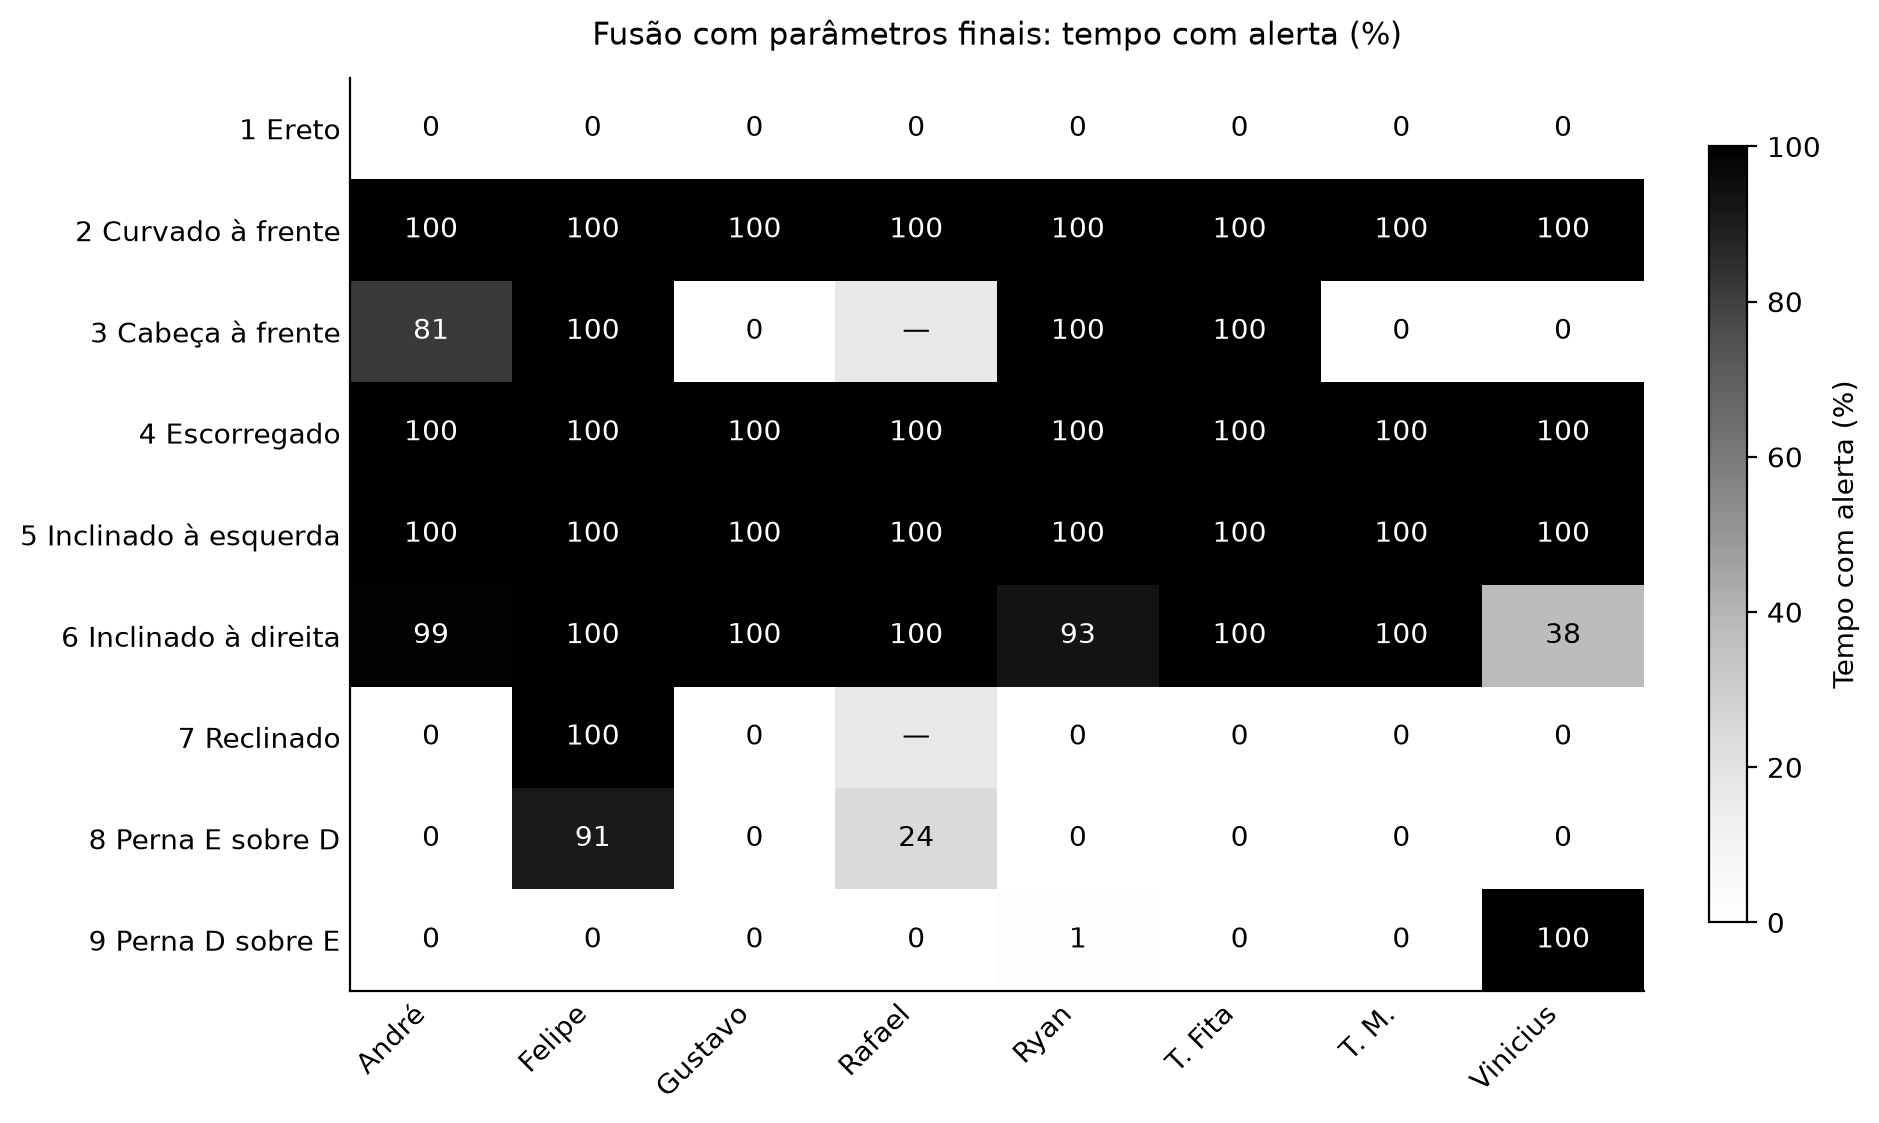
\includegraphics[width=\linewidth]{res_alerta_sujeitos.png}
  \fonte{Elaborado pelo autor (2026)}
  \par\smallskip
  {\footnotesize Percentuais ponderados pelo número de amostras estabilizadas.
  Espera-se alerta nas linhas 2--6 e ausência de alerta nas demais. Traço:
  postura não registrada.}
\end{figure}

A postura curvada para frente permaneceu alertada em todo o tempo avaliado
pelas três regras. O escorregamento passou de $72\,\%$ para $100\,\%$ com a
fusão final: a leitura do assento recuperou casos em que o tronco quase não
inclinou, como Rafael e parte das passagens de Thiago Fita. A inclinação à
esquerda passou de $94\,\%$ para $100\,\%$, incluindo o movimento de pequena
amplitude de Felipe. O reclinado apresentou a maior redução de falso alarme,
de $78\,\%$ para $5\,\%$ do tempo. O único segmento reclinado ainda alertado
com os parâmetros finais foi o de Felipe.

A pontuação de Vinicius passou de $0{,}67$ para $0{,}74$, mantida em LOSO;
a de Felipe passou de $0{,}68$ para $0{,}76$, caindo para $0{,}71$ em LOSO.
Ryan e Thiago Fita ficaram próximos de um com a fusão final. Portanto, o
resultado agregado não representa desempenho uniforme entre usuários.

\subsubsection{Contribuição de cada componente e cadeira vazia}

A ablação cumulativa, apresentada na Figura~\ref{fig:res-ablacao}, manteve os
parâmetros finais e ativou sucessivamente os componentes. A pontuação passou
de $0{,}834$ na regra só-IMU para $0{,}850$ com a detecção de escorregamento,
$0{,}922$ com o tratamento de reclinação e $0{,}935$ com a confirmação
lateral. O maior incremento correspondeu a deixar de penalizar a inclinação
para trás quando o apoio traseiro permanecia presente. Por ser uma ablação
cumulativa, os incrementos dependem da ordem de inclusão e não representam
contribuições estatisticamente independentes.

\begin{figure}[H]
  \centering
  \caption{Ablação cumulativa da regra de alerta com os parâmetros finais.}
  \label{fig:res-ablacao}
  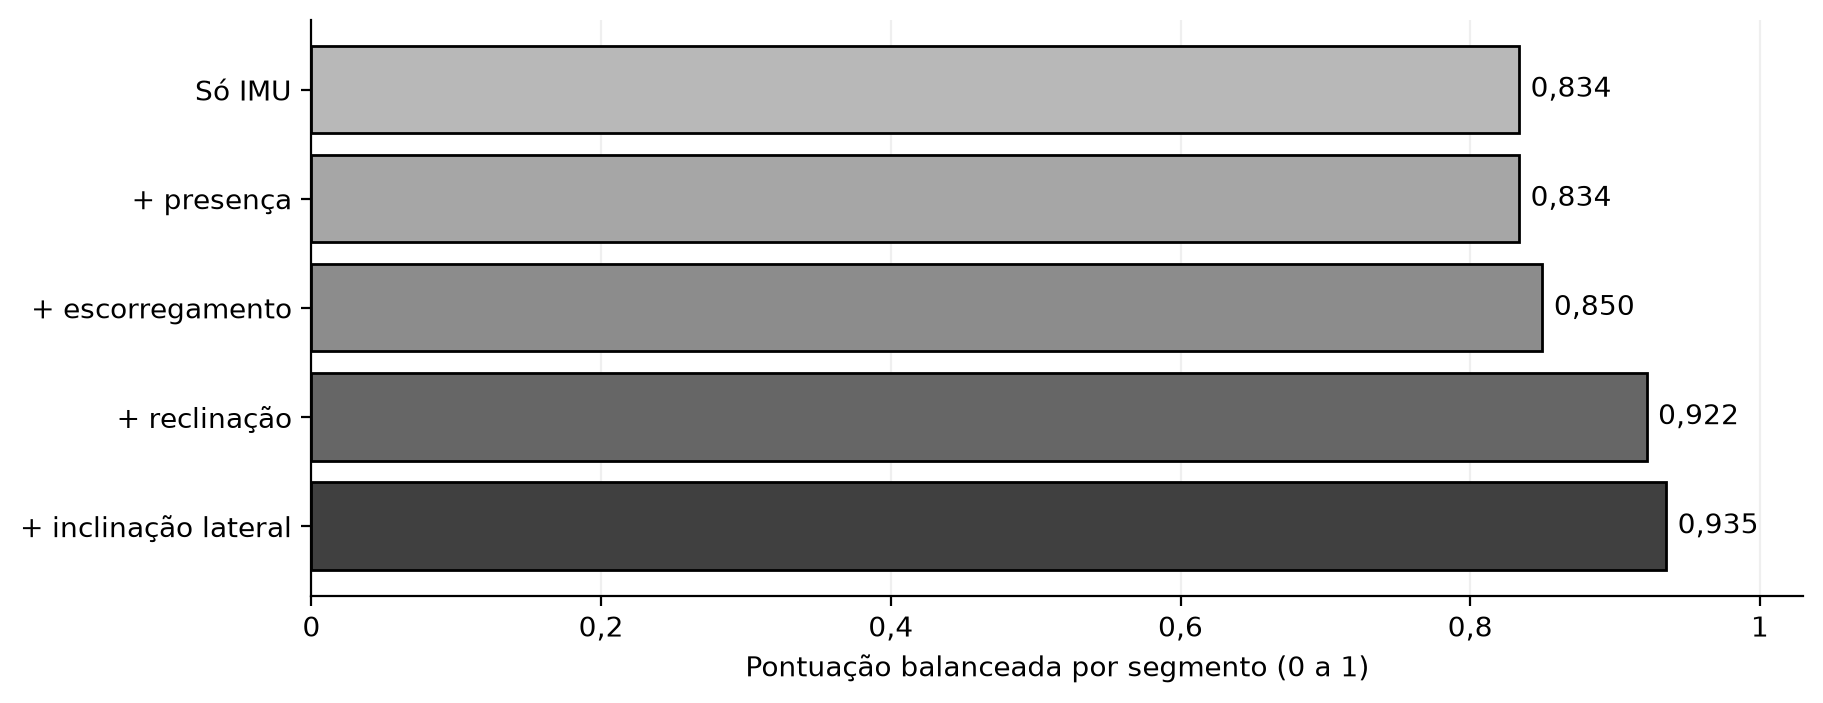
\includegraphics[width=0.98\linewidth]{res_ablacao.png}
  \fonte{Elaborado pelo autor (2026)}
\end{figure}

A supressão por presença não alterou a pontuação dos segmentos sentados,
mas evitou alertas nos intervalos de cadeira vazia. Com soma do assento
inferior a 2000 contagens, houve 176{,}30\,s de vazio: a referência alertou
em 70{,}85\,s e a fusão em 0\,s, aproximadamente os 176\,s e
71\,s documentados. Nesses intervalos, a pessoa podia estar em pé com o
colar; seu desvio inercial não indicava postura sentada inadequada.

\subsubsection{Falhas conhecidas, pernas cruzadas e limites temporais}

Na postura de cabeça à frente, Gustavo, Thiago M. e Vinicius não receberam
alerta. São três participantes entre os oito do conjunto, mas apenas sete
realizaram essa postura. A inclinação medida na região superior das costas
foi pequena e o contato com a cadeira permaneceu semelhante ao ereto. A fusão
não recuperou esses movimentos: o tempo alertado agregado continuou em
$70\,\%$. Reduzir o limiar frontal aproximaria a decisão do ereto de Rafael,
cujo percentil 5 de \texttt{droll} chegou a cerca de $-7{,}5\degree{}$.
Portanto, a falha não se resolve nos dados apenas supondo que os FSRs sempre
complementam um sinal inercial insuficiente.

Em Felipe, \texttt{dpitch} permaneceu próximo de $+10\degree{}$ após a
inclinação à direita. O reclinado alertou em $100\,\%$ do tempo e a perna
esquerda cruzada em $91\,\%$, sem mudança correspondente no assento.
A análise interpreta o padrão como deriva mecânica do colar ou da referência,
não como integração do giroscópio. A calibração inicial não assegura
estabilidade da fixação durante toda a sessão.

A inclinação à direita de Vinicius alertou em apenas $38\,\%$ do tempo:
o desvio ficou próximo do limiar e o assento deslocou no sentido oposto à
confirmação lateral. Também ocorreram posturas mistas: Vinicius escorregou
no código 9, gerando um alerta fisicamente justificável, mas contado como
falso alarme pela etiqueta; Ryan permaneceu escorregado no código 5,
continuando corretamente detectado. A classe dominante pode divergir da
etiqueta sem invalidar a detecção.

O cruzamento das pernas não apresentou padrão de pressão suficientemente
comum entre sujeitos. O módulo do deslocamento lateral excedeu $0{,}1$ em
apenas três dos oito participantes na postura 8; houve alterações por outros
índices na postura 9, mas sem direção consistente entre pessoas.
Com os parâmetros finais, os códigos 8 e 9 tiveram $12\,\%$ e $10\,\%$
do tempo alertado. Em Rafael, o código 8 apresentou $24\,\%$ de alerta por
confirmação lateral (Figura~\ref{fig:res-alerta-sujeitos}): a perna cruzada
deslocou a carga do assento enquanto o colar registrava inclinação lateral
próxima de $-5{,}7\degree{}$. A opção de não alertar
por pernas cruzadas corresponde ao escopo da regra avaliada, não a uma
conclusão clínica sobre essa posição.

O LOSO tornou algumas margens mais visíveis. Sem Thiago Fita, a escolha de
limiar traseiro $0{,}5$ passou a alertar sua postura 9, cuja razão traseira
foi de aproximadamente $0{,}40$. Sem Gustavo, o limiar de reclinação
$0{,}5$ reduziu a detecção do seu escorregamento a $23\,\%$ do tempo;
nesse caso a razão traseira era aproximadamente $0{,}49$. Sem André,
o limiar angular escolhido caiu para $8\degree{}$ e passou a gerar alertas
em trechos com pernas cruzadas e deslocamento lateral da referência.
Esses casos explicam a elevação de falso alarme nas pernas cruzadas em LOSO,
mesmo com manutenção do total de segmentos prejudiciais detectados.

Alerta em ao menos uma amostra não implica aviso sustentado. A histerese
pode transportar um alerta anterior se o desvio permanecer entre
$7\degree{}$ e $10\degree{}$. Latência zero desde a tecla também não
significa resposta instantânea: a pessoa frequentemente já havia cumprido
a espera de 3\,s durante a transição. A latência entre início físico do
movimento e vibração não foi medida.

\subsection{Validação em hardware em 22 de outubro de 2026}
\label{sec:res-hardware}

\subsubsection{Rodada guiada com participante já conhecido}

A primeira validação utilizou André, já presente no desenvolvimento, com
fusão nas placas e motor ativo (versão \texttt{c4ae8f2}). A rodada guiada,
com retenções de cerca de 16\,s, incluiu cadeira vazia, recolocação do
colar e recalibração. Os códigos 2--6 alertaram em $100\,\%$ do tempo
estabilizado; 1, 7, 8 e 9, em $0\,\%$. Os seis segmentos prejudiciais foram
detectados, incluindo duas ocorrências de escorregamento.

O participante percebeu a vibração e sua interrupção ao retornar ao ereto.
Não houve perda de pacotes nem indicação de falha do IMU. Verificou-se o
percurso entre sensores, decisão na cadeira, enlace e atuação corporal,
sem representar teste com pessoa nova ou medida de latência. Os detalhes de
ajuste do colar e da cadeira não foram registrados.

\subsubsection{Primeiro participante não utilizado no desenvolvimento}

Lucas Santos foi o primeiro participante sem dados nas capturas utilizadas
para escolher a regra. A sessão empregou a versão \texttt{b3c29b1}, com
protocolo de comunicação v5 e motor ativo. O roteiro foi parcial: ereto,
inclinado à esquerda, escorregado, perna esquerda sobre a direita, ereto,
curvado à frente e inclinado à direita, seguido de aproximadamente 10\,s
de cadeira vazia. Não foram realizadas as posturas 3, 7 e 9, a segunda
passagem, os movimentos sutis nem a recolocação do colar. Houve uma calibração,
sem perda de pacotes e sem indicação de falha do IMU.

A Tabela~\ref{tab:res-validacao} compara as duas sessões usando o alerta
registrado pelo firmware, e não uma previsão substituída pela reprodução.
Na sessão de Lucas, curvar para frente e escorregar produziram alerta em
$100\,\%$ do tempo estabilizado; ereto e cadeira vazia não produziram
alerta. Três problemas impediram a reprodução do resultado da rodada guiada:
instabilidade do alerta durante a vibração, perda da inclinação à direita
e alertas curtos com perna cruzada.

\begin{table}[H]
  \centering
  \caption{Tempo estabilizado com alerta registrado nas duas sessões de
  validação em hardware de 22/10/2026.}
  \label{tab:res-validacao}
  \begin{singlespace}
  \begin{tabularx}{\linewidth}{cXrr}
    \toprule
    Código & Postura & André (\%) & Lucas (\%) \\
    \midrule
    1 & Ereto                & 0 & 0 \\
    2 & Curvado à frente     & 100 & 100 \\
    3 & Cabeça à frente      & 100 & --- \\
    4 & Escorregado          & 100 & 100 \\
    5 & Inclinado à esquerda & 100 & $9{,}2$ \\
    6 & Inclinado à direita  & 100 & 0 \\
    7 & Reclinado            & 0 & --- \\
    8 & Perna E sobre D      & 0 & $2{,}9$ \\
    9 & Perna D sobre E      & 0 & --- \\
    \bottomrule
  \end{tabularx}
  \fonte{Elaborado pelo autor (2026)}
  \end{singlespace}
  \par\smallskip
  {\footnotesize Excluídos os primeiros 2\,s de cada segmento, como na
  avaliação anterior. Traço: postura não realizada. Os valores de Lucas
  para os códigos 5 e 8 são $11{,}6\,\%$ e $2{,}6\,\%$, respectivamente,
  quando se considera todo o intervalo rotulado, sem essa exclusão.}
\end{table}

A Figura~\ref{fig:res-validacao-lucas} mostra a perda de apoio traseiro no
escorregamento, detectado mesmo com desvio frequentemente abaixo de
$10\degree{}$, e o alerta sustentado na curvatura à frente. A inclinação
à direita não satisfez os critérios.

\begin{figure}[H]
  \centering
  \caption{Linha do tempo da sessão de Lucas: desvio registrado pela cadeira,
  razão traseira do assento, alerta registrado e etiqueta da postura.}
  \label{fig:res-validacao-lucas}
  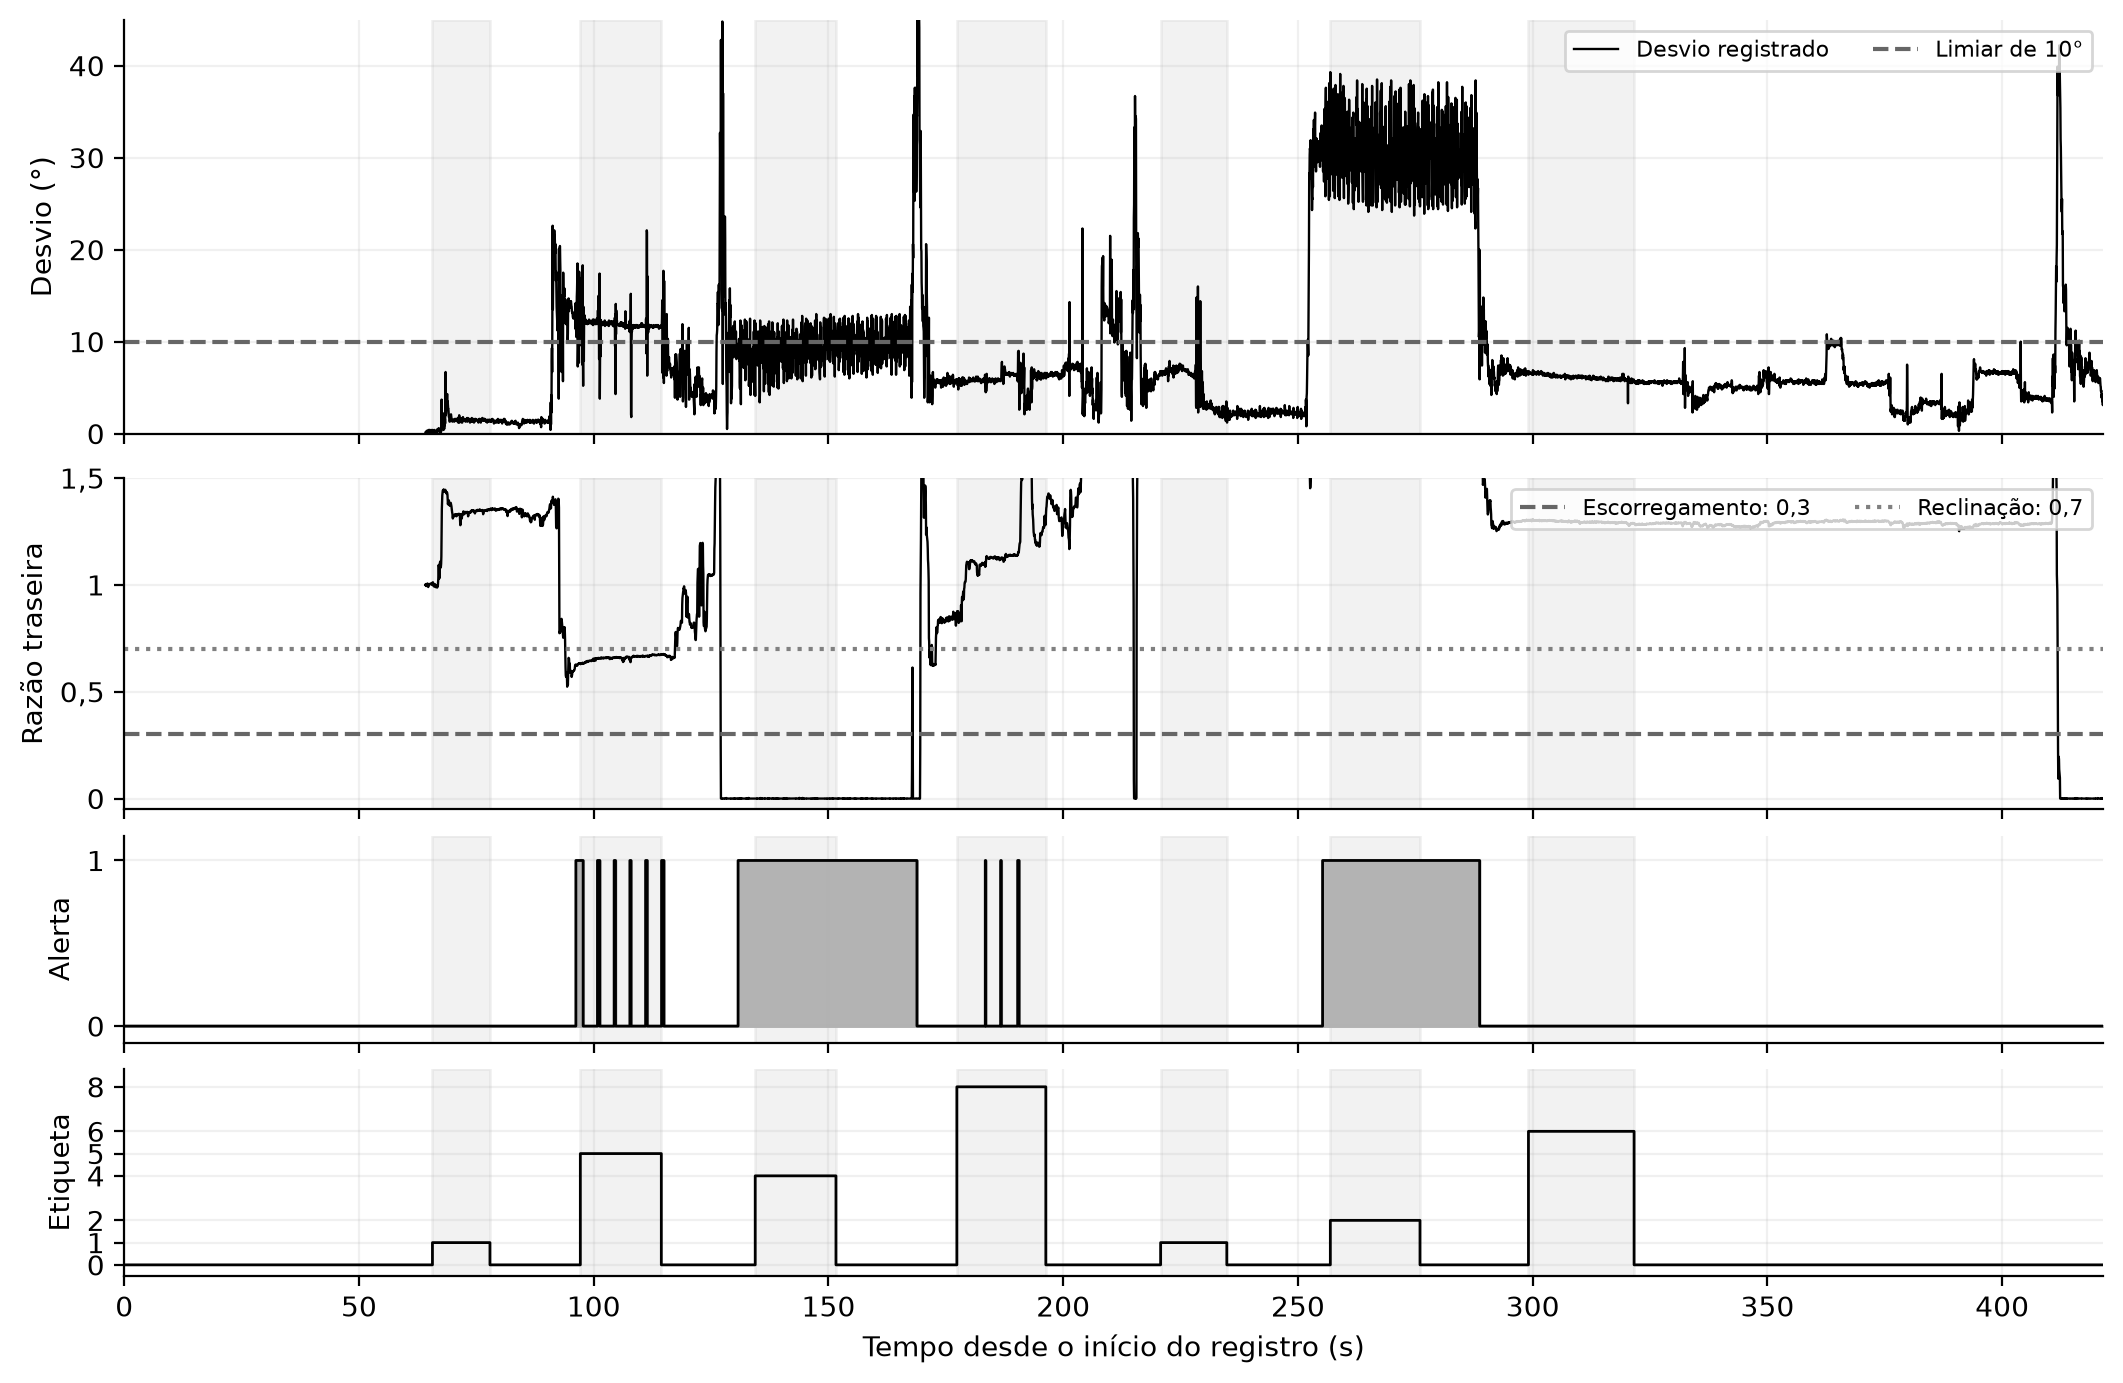
\includegraphics[width=\linewidth]{res_validacao_lucas.png}
  \fonte{Elaborado pelo autor (2026)}
  \par\smallskip
  {\footnotesize As faixas cinza indicam intervalos rotulados; etiqueta zero
  indica transição ou intervalo sem postura marcada. A leitura anterior à
  calibração não é mostrada nos dois primeiros painéis. Os eixos de desvio e
  razão traseira são limitados para favorecer a leitura das posturas mantidas;
  picos de movimento podem ultrapassar esses limites.}
\end{figure}

Na inclinação à esquerda, o desvio ficou próximo de $12\degree{}$ e a
condição de postura inadequada esteve presente entre os pulsos do motor.
Entretanto, o início da vibração provocou oscilações da ordem de
$\pm10\degree{}$ no IMU, com amostras abaixo do limiar de limpeza de
$7\degree{}$. Cada limpeza exigiu nova permanência de 3\,s para reativar
o alerta. A Figura~\ref{fig:res-motor-lucas} mostra as quedas abruptas do
desvio próximas aos pulsos reportados pelo corpo. O registro da análise
identificou seis reinícios desse tipo, produzindo avisos breves em vez de
uma sequência sustentada de vibração.

\begin{figure}[H]
  \centering
  \caption{Interferência da vibração na inclinação à esquerda de Lucas:
  oscilações do desvio, limiares e interrupções do alerta.}
  \label{fig:res-motor-lucas}
  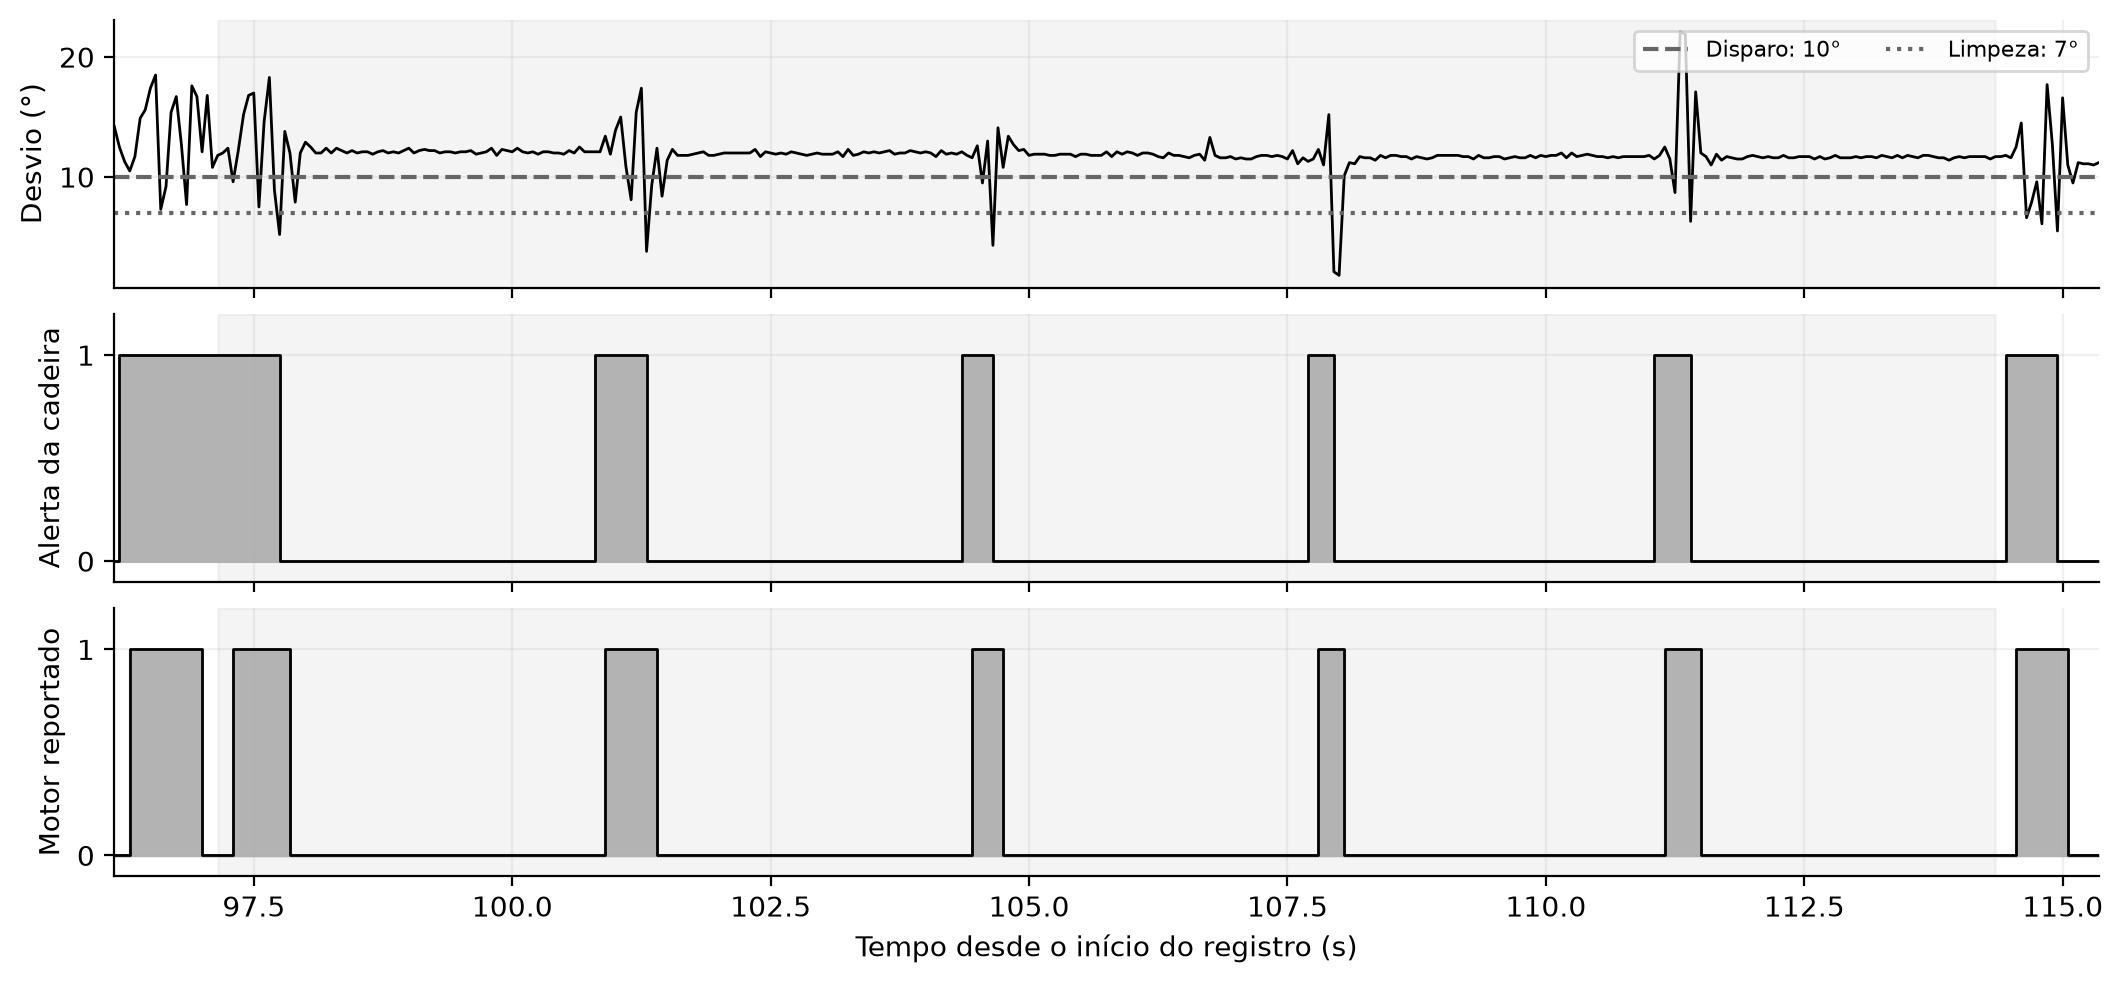
\includegraphics[width=\linewidth]{res_motor_lucas.png}
  \fonte{Elaborado pelo autor (2026)}
  \par\smallskip
  {\footnotesize O painel inferior apresenta o estado de motor reportado
  pelo corpo na coluna \texttt{bmotor}, e não uma medição elétrica do atuador.
  A faixa cinza corresponde ao segmento com etiqueta 5.}
\end{figure}

Considerando todo o segmento rotulado, o firmware alertou em
$11{,}6\,\%$ das amostras, valor arredondado para $12\,\%$ no registro
da sessão. Excluindo seus primeiros 2\,s, o valor foi $9{,}2\,\%$.
A reprodução atual fornece os mesmos $9{,}2\,\%$ nesse recorte; portanto,
a diferença entre ``12\,\% registrado'' e ``9\,\% reproduzido'' citada no
registro não se mantém ao igualar o denominador. Na postura 8, por outro
lado, o alerta registrado foi $2{,}9\,\%$ do tempo estabilizado, enquanto
a reprodução retornou $7{,}7\,\%$. Conserva-se o valor registrado na tabela
de hardware; a reprodução de ângulos arredondados em movimentos próximos aos
limiares não substitui o estado efetivamente executado nas placas.

A inclinação à direita de Lucas foi perdida: \texttt{dpitch} ficou próximo
de $+5{,}5\degree{}$, com redistribuição do assento para a esquerda,
contrária à condição de confirmação. O desvio lateral do segundo ereto
havia mudado aproximadamente $3{,}5\degree{}$ para a esquerda em relação
à referência inicial. Já a postura 8 produziu três alertas curtos associados
à condição lateral, com \texttt{dpitch} próximo de $-5{,}5\degree{}$, junto
à fronteira de $5\degree{}$. Os dois casos mostram que movimento do colar
e deslocamento causado pelas pernas podem aproximar posturas diferentes da
mesma fronteira de decisão.

\subsubsection{Correção posterior da interferência do atuador}

O histórico do firmware registra uma correção após essa validação, no
\textit{commit} \texttt{5e82e20}: enquanto o PWM do motor está ativo, o corpo
transmite a última leitura válida obtida com o motor desligado, evitando
substituí-la por uma leitura perturbada pela vibração. O limite dessa
retenção foi posteriormente ampliado para 1{,}5\,s no
\textit{commit} \texttt{6eaafbe}. A regra de fusão da cadeira permaneceu
inalterada.

A mensagem da correção relata uma reprodução com retenção dos ângulos em que
o alerta da inclinação à esquerda de Lucas passou de cerca de $9\,\%$ para
$100\,\%$, com mudança de aproximadamente $8\,\%$ para $11\,\%$ nas
pernas cruzadas e sem alteração no resultado de André. Esses números são
uma verificação por reprodução registrada no histórico, não uma nova sessão
física. Os dois arquivos de validação disponíveis foram obtidos com versões
anteriores à correção; não há nova captura registrada que confirme em hardware
o efeito da retenção. A demonstração posterior na feira, descrita a seguir,
fornece apenas evidência qualitativa e não supre essa comparação controlada.

\subsection{Demonstração na feira de ciências em novembro de 2026}
\label{sec:res-feira}

Na feira de ciências, dezenas de pessoas utilizaram cadeira instrumentada,
unidade corporal e alerta por vibração. Segundo o relato registrado no
projeto, a postura prejudicial foi detectada em praticamente todos os casos
observados. Houve nomes de postura divergentes do esperado em movimentos
combinados, mesmo com detecção da condição para alerta.

Sem arquivos das sessões, contagens de erros ou sequência padronizada,
não se calculam sensibilidade, especificidade ou taxa de acerto para a feira.
A evidência é qualitativa de funcionamento com várias pessoas fora da rodada
de desenvolvimento. Não se mediram mudança de hábito, redução de dor ou
benefício clínico.

\subsection{Enlace de comunicação e energia}
\label{sec:res-enlace-energia}

\subsubsection{Enlace ESB e monitoramento por beacon BLE}

No ensaio de bancada do enlace corpo--cadeira, a aproximadamente 1\,m, não
houve pacotes perdidos na taxa de 20\,Hz. Após a decisão ser transferida
para a cadeira e devolvida na carga útil de confirmação, foram observadas
aproximadamente 10--35 retransmissões por segundo. Portanto, ausência de
perda ao final das tentativas não significa ausência de repetição no rádio.
As sessões de validação de 22/10 também registraram zero perda de pacotes.
Esses resultados caracterizam os ensaios disponíveis, sem estabelecer alcance
máximo ou robustez sob outras condições de interferência.

O ensaio específico do \textit{beacon} BLE teve 60\,s de duração, com as
duas placas alimentadas por USB e recepção em um notebook com interface
MediaTek. Foram transmitidos 1200 anúncios e recebidos 225, correspondentes
a $3{,}75$ recepções por segundo e $18{,}75\,\%$ dos anúncios enviados.
A Tabela~\ref{tab:res-ble} sintetiza as lacunas. Os 225 registros recebidos
concordaram com os dados USB, com diferença de relógio de 0--1\,ms.
Nesse ensaio específico, o ESB manteve $20$ amostras por segundo, sem perda,
duplicação, pacotes inválidos, retransmissões ou entrada em modo de decisão
local por perda de enlace.

\begin{table}[H]
  \centering
  \caption{Recepção do beacon BLE no ensaio de bancada de 60 segundos.}
  \label{tab:res-ble}
  \begin{singlespace}
  \begin{tabularx}{\linewidth}{Xr}
    \toprule
    Indicador & Resultado \\
    \midrule
    Anúncios enviados / recebidos & 1200 / 225 \\
    Fração recebida & $18{,}75\,\%$ \\
    Taxa média de recepção & 3{,}75\,s$^{-1}$ \\
    Intensidade de sinal aproximada & $-73$\,dBm \\
    Mediana dos intervalos entre recepções & 175{,}5\,ms \\
    Percentil 90 dos intervalos & 500\,ms \\
    Maior intervalo & 1{,}9\,s \\
    \bottomrule
  \end{tabularx}
  \fonte{Elaborado pelo autor (2026)}
  \end{singlespace}
\end{table}

Os ensaios ESB com e sem retransmissões são observações distintas, sem
comparação controlada que explique a diferença ou encerre a questão.
O BLE permitiu exibir o estado recebido, mas suas lacunas impedem uma
captura completa. A decisão permanece autônoma pelo ESB; o notebook recebe
uma cópia. Os arquivos analisados neste capítulo foram obtidos por USB.

\subsubsection{Alimentação por bateria e medidas ainda ausentes}

O projeto registra funcionamento do corpo com LiPo e teste funcional
posterior da cadeira com o mesmo circuito. A célula corporal JYH LIP103450
é rotulada como 1800\,mAh e 3{,}7\,V; são especificações nominais, não
medidas de capacidade útil. O funcionamento sem USB não quantifica duração
da carga nem estabilidade do rádio durante a descarga.

No corpo, três leituras abaixo de 3{,}30\,V, sem USB e com motor desligado,
acionam \textit{System OFF}; a inicialização por bateria exige
3{,}40\,V. São limiares implementados, sem curva de descarga ou ensaio
completo registrado de corte e despertar por USB. O teste do beacon foi
alimentado por USB e não caracteriza seu consumo em bateria.

A pesquisa de alimentação registra correntes nominais de carga de $50$ ou
100\,mA e temporizador de segurança de aproximadamente dez horas.
Não se demonstrou carga completa em uma conexão ao USB, nem se mediram
tempo de recarga e energia reposta. Especificações de componentes não
fundamentam uma autonomia medida.

\pendente{Medir a corrente consumida por corpo e cadeira, discriminando
repouso operacional, comunicação e acionamento do motor, e registrando as
condições de alimentação e do beacon BLE.}

\pendente{Medir a autonomia de cada unidade por ciclo de descarga, com tensão
inicial, critério de término, padrão de alertas e condição do enlace
registrados; a capacidade nominal da bateria não substitui essa medição.}

% RASTREABILIDADE PARA INTEGRACAO (nao aparece no PDF):
% Bancada: report/relatorio_parcial.tex; analysis/archive/VALIDATION.md;
% analysis/archive/FSR_FINDINGS.md. As figuras antigas sao reaproveitadas.
% Conjunto: data/README.md; captures.py; execucao de report_figures.py.
% Fusao: docs/decisao-fusao-imu-fsr.md; execucao integral de fusion.py.
% Rafael tag 8: 24% com fusao (doc: celula '0/24' = atual/fusao).
% Lucas tag 5: log e replay = 11,594% integral, 9,180% estabilizado;
% registro compara 12% log a 9% replay sem igualar o denominador.
% Lucas tag 8: log estabilizado 2,950%, replay 7,670%; usa-se log em hardware.
% Correcao do motor: git show 5e82e20 e 6eaafbe; sem CSV posterior de validacao.
% Feira e bateria funcional das duas unidades: AGENTS.md (status nov/2026).
% ESB: AGENTS.md e TASKS.md; BLE: firmware/README.md.
% Energia: docs/pesquisa-bateria-lipo.md e firmware/README.md.
% Sem referencias bibliograficas novas; fontes internas de resultados proprios.
